\documentclass{article}
\usepackage[english]{babel}
\usepackage[utf8]{inputenc}
\usepackage{algorithm}
\usepackage[noend]{algpseudocode}
\usepackage{amsmath,amsfonts,amsthm}
\usepackage{lipsum}
\usepackage{tikz}
\usepackage{tikz-cd}
\usepackage{tikz-qtree}
\usepackage{graphicx}
\usepackage{placeins}
\usetikzlibrary{shapes.geometric, positioning}

\usepackage[letterpaper, margin=1.25in]{geometry}

\title{Book Store Requirements, Architecture, and Patterns}
\author{Dakota Wynn\\
		Lucas Bramer\\
		Jason Reid\\
	Software Design and Architecture\\
	University of Central Missouri -- UCM}
\date{\today}

\begin{document}
	
	\maketitle
	
	% Body
	\section*{Project Scope:}
	User will be able to browse a books catalog. \\
	User will be able to register and login. \\
	User will be able to manage an individual cart before placing an order. \\
	User will be able to simulate payment and ordering. \\
	Admin will be able to  add/update books. \\
	Stretch: User will be notified when order is placed. \\
	
	
	\section*{Architecture + Requirements: Three-Tiered}
	Frontend: Vue, JS, HTML/CSS, Node \\
	Backend: Django, Python \\
	Database: MySQL, AWS RDS \\
	
	\newpage
	
	\section*{Entity Relationship Diagram:}
	\begin{figure}[h]
		\centering
		\includegraphics[width=1\textwidth]{Bookstore_ERD.png}
		\caption{Entity Relationship Diagram}
		\label{fig:ERD}
	\end{figure}
	\FloatBarrier
	
	\section*{ERD and Database Explained:}
	User -owns→ Cart -contains→ CartItem -adds→ Books \\
	Cart -converts→ Order -complete→ Payment \\
	User -places→ Order \\
	
	\section*{Patterns Definitions:}
	Singleton: Ensures a class has only one instance, and provides a global point of access to it.\\
	Strategy: Defines a family of algorithms, encapsulates each one, and makes them interchangeable. \\
	Factory: Defines an interface for creating an object, but lets sub-classes decide which class to instantiate. Factory method lets a class defer instantiation to sub-classes. \\
	Observer: Defines a one-to-many dependency between objects so that when one object changes state, all its dependents are notified and updated automatically. \\
	State: Allow an object to alter behavior when its internal state changes. It will appear to change its class.\\
	
	\newpage
	
	\section*{Unified Modeling Language (UMLs):}
	\begin{figure}[h]
		\centering
		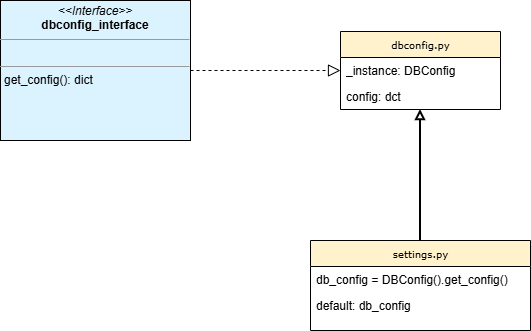
\includegraphics[width=1\textwidth]{SingletonUML.png}
		\caption{Singleton UML Diagram}
		\label{fig:Singleton}
	\end{figure}
	\FloatBarrier
		\begin{figure}[h]
		\centering
		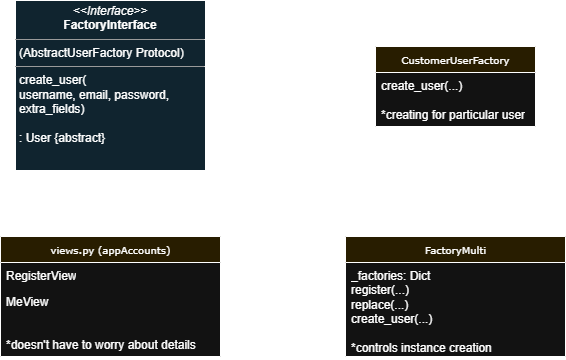
\includegraphics[width=1\textwidth]{FactoryUML.png}
		\caption{Factory UML Diagram}
		\label{fig:Factory}
	\end{figure}
	\FloatBarrier
	\section*{UMLs Explained:}
	Singleton: Uses the dbconfig-interface to set what is required. Separates the instances of db connection so that there is only one instance and any given time in dbconfig.py. Then settings.py in mysite will be able to use strictly one instance. \\
	Factory: Uses the factory-interface to set what is required. The customer-user-factory is the concrete class that has rules in creating a user for the customer. The factory-multi class will control the instance creation. Then the views class from appAccounts will be able to create users without knowing the details\\

	
	\newpage
	
	\section*{Challenges: }
	Research: The biggest undertaking with reasearch was understanding what we did not need. There was a vast array of different sources all telling you more than what you needed to use. Understanding what we have learned in class as far as what good software design is, helped us understand what was useful for the scope of the project. \\
	Database: Setting up the database correctly with connection accross all teammates. Using RDS AWS was a solution we found so that the database would update constantly. Furthermore, it wasn't until we correctly setup the ERD that the database and the rest of development went smoothly. Having correct data interaction was crucial for the success of the project.\\
	Backend: Learning all the different intricacies of Django and Python and what it had to offer was a huge undertaking. Understanding the relations between what views, serializers, models, etc are.  \\
	Frontend: Learning how to use Vue's framework model of script,template, and css. Having all of them in one class eventually made it easier; however, learning how to route them correctly to the default skeleton Vue made was challenging to understand. Eventually with research, learning routers help with this issue.  \\
	
	\section*{Future Implementations:}
	Updated Catalog: Add more books, options, and stock \\
	Text Updates: Try implementing text updates instead and updating the order state implementation to correctly update states. \\
	2FA/SSO: Implement a more secure login system with 2FA or SSO.\\
	Payment System Actualized: Having an implementation of payment system working and also verifying failed payments.\\
	
	\section*{Research References:}
	https://app.diagrams.net/ (draw.io for umls) \\
	https://docs.aws.amazon.com/AmazonRDS/latest/AuroraUserGuide/Aurora.AuroraMySQL.html \\
	https://getbootstrap.com/ and frontend AI implemenations\\
	python, vue, mysql, django single syntax searches \\
	https://www.w3schools.com/django/djangomodels.php \\
	https://erdplus.com/ (for erd creation)\\
	https://www.geeksforgeeks.org/python/modelserializer-in-serializers-django-rest-framework/ \\
	https://www.geeksforgeeks.org/techtips/enabling-third-party-app-login-using-google-account/ \\
	
	
	
\end{document}